%Other relevant parameters for the TRITIUM monitor are the PDE, which determines the minimum detectable activity (MDA), the dark count rate and the crosstalk probability, which generate fake counts. They were not measured since it was not possible with the current setup. It is expected to be measured for the S13360-6075 model, the latest proposal for the TRITIUM detector, where all the relevant parameters will be experimentaly determined using a different experimental setup, described in appendix \ref{App:ElectronicReadoutSiPM}.
The characterization the most relevant paramenter of the SiPM S13360-1375 from Hamamatsu, which was the first choice for the TRITIUM monitor photosensor, are described in this section. The most relevant SiPM paramenters are breakdown voltage $V_{BD}$, SiPM gain and the gain dependence on operating voltage and temperature $G_{SiPM}(V_{bias}, T)$ and temperature coeficient $e$. Additional parameters were measured to verify the accuracy of the characterization such as the quenching resistance $R_q$, the pixel capacitance $C_d$, and the terminal capacitance $C_t$. The afterpulse probability was not measured since, as reported in seccion \ref{sec:MonitorOverview}, it is negligible when time coincidence windows of $10~\ns$ are employed. The SiPM characterization was carried out inside of a climatic chamber, model CCM 81 from DYCOMETAL \cite{ClimaticChamberIFIMED}. This climatic chamber allows to control both temperature and humidity with a precision of $0.1\celsius$ and $0.1\%$ respectively. In addition, this chamber works as a Faraday cage. A special black blanket \cite{BlackBlancket} screened the SiPM from external. 

The quenching resistance and the breakdown voltage were measured from the output current of the SiPM as a function of its forward and reverse bias voltage, respectively. The output current of the SiPM was measured by a Keithley 6487 Picoammeter/Voltage Source \cite{DataSheetKeithley6487}. The LabView sofware was used to take the data. The current-voltage curves are shown in Figure \ref{fig:IVcurveSiPM}.
\begin{figure}
\centering
    \begin{subfigure}[b]{0.9\textwidth}
    \centering
    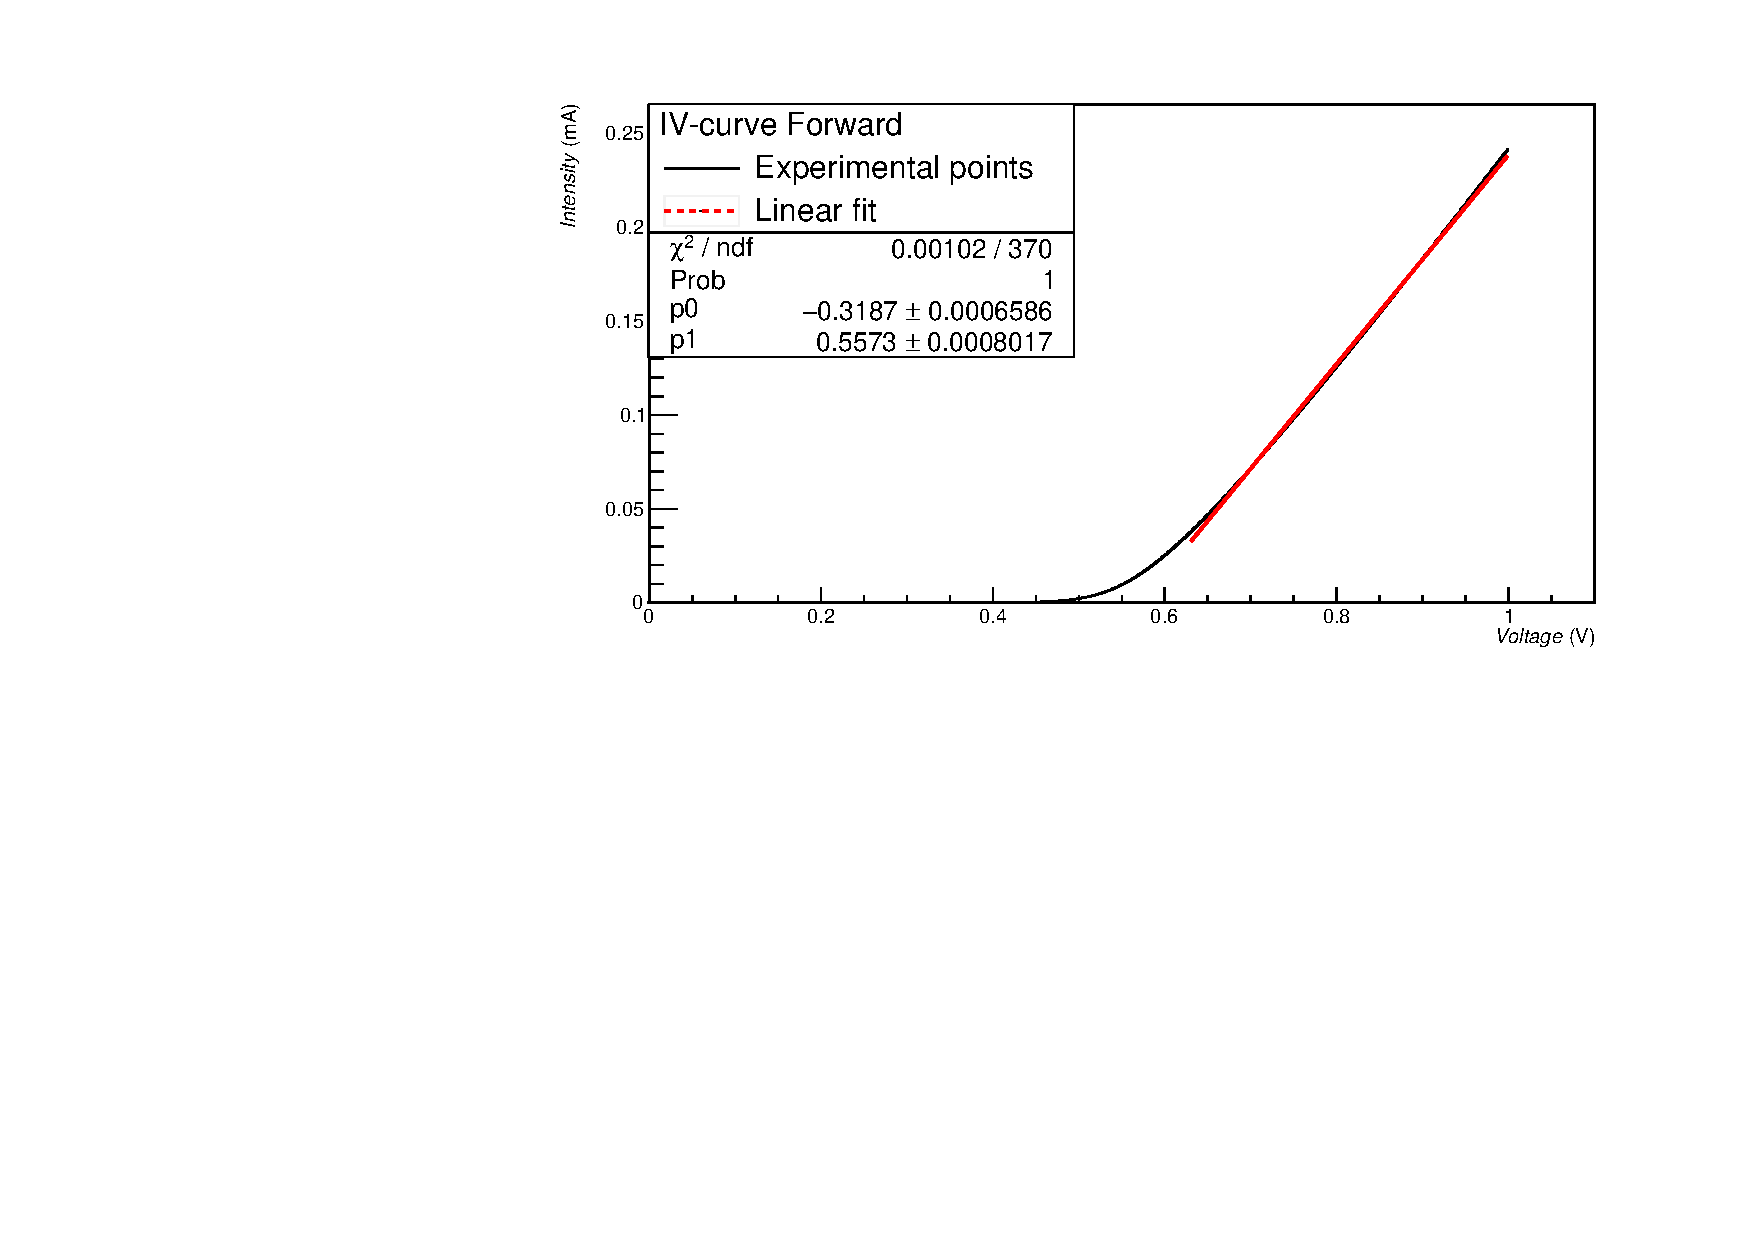
\includegraphics[width=\textwidth]{4ResearchAndDevelopments/42SiPM/IVCurveSiPMForward.pdf}  
    \caption{\label{subfig:IVcurveForward}}
    \end{subfigure}
    \hfill
    \begin{subfigure}[b]{0.9\textwidth}
    \centering
    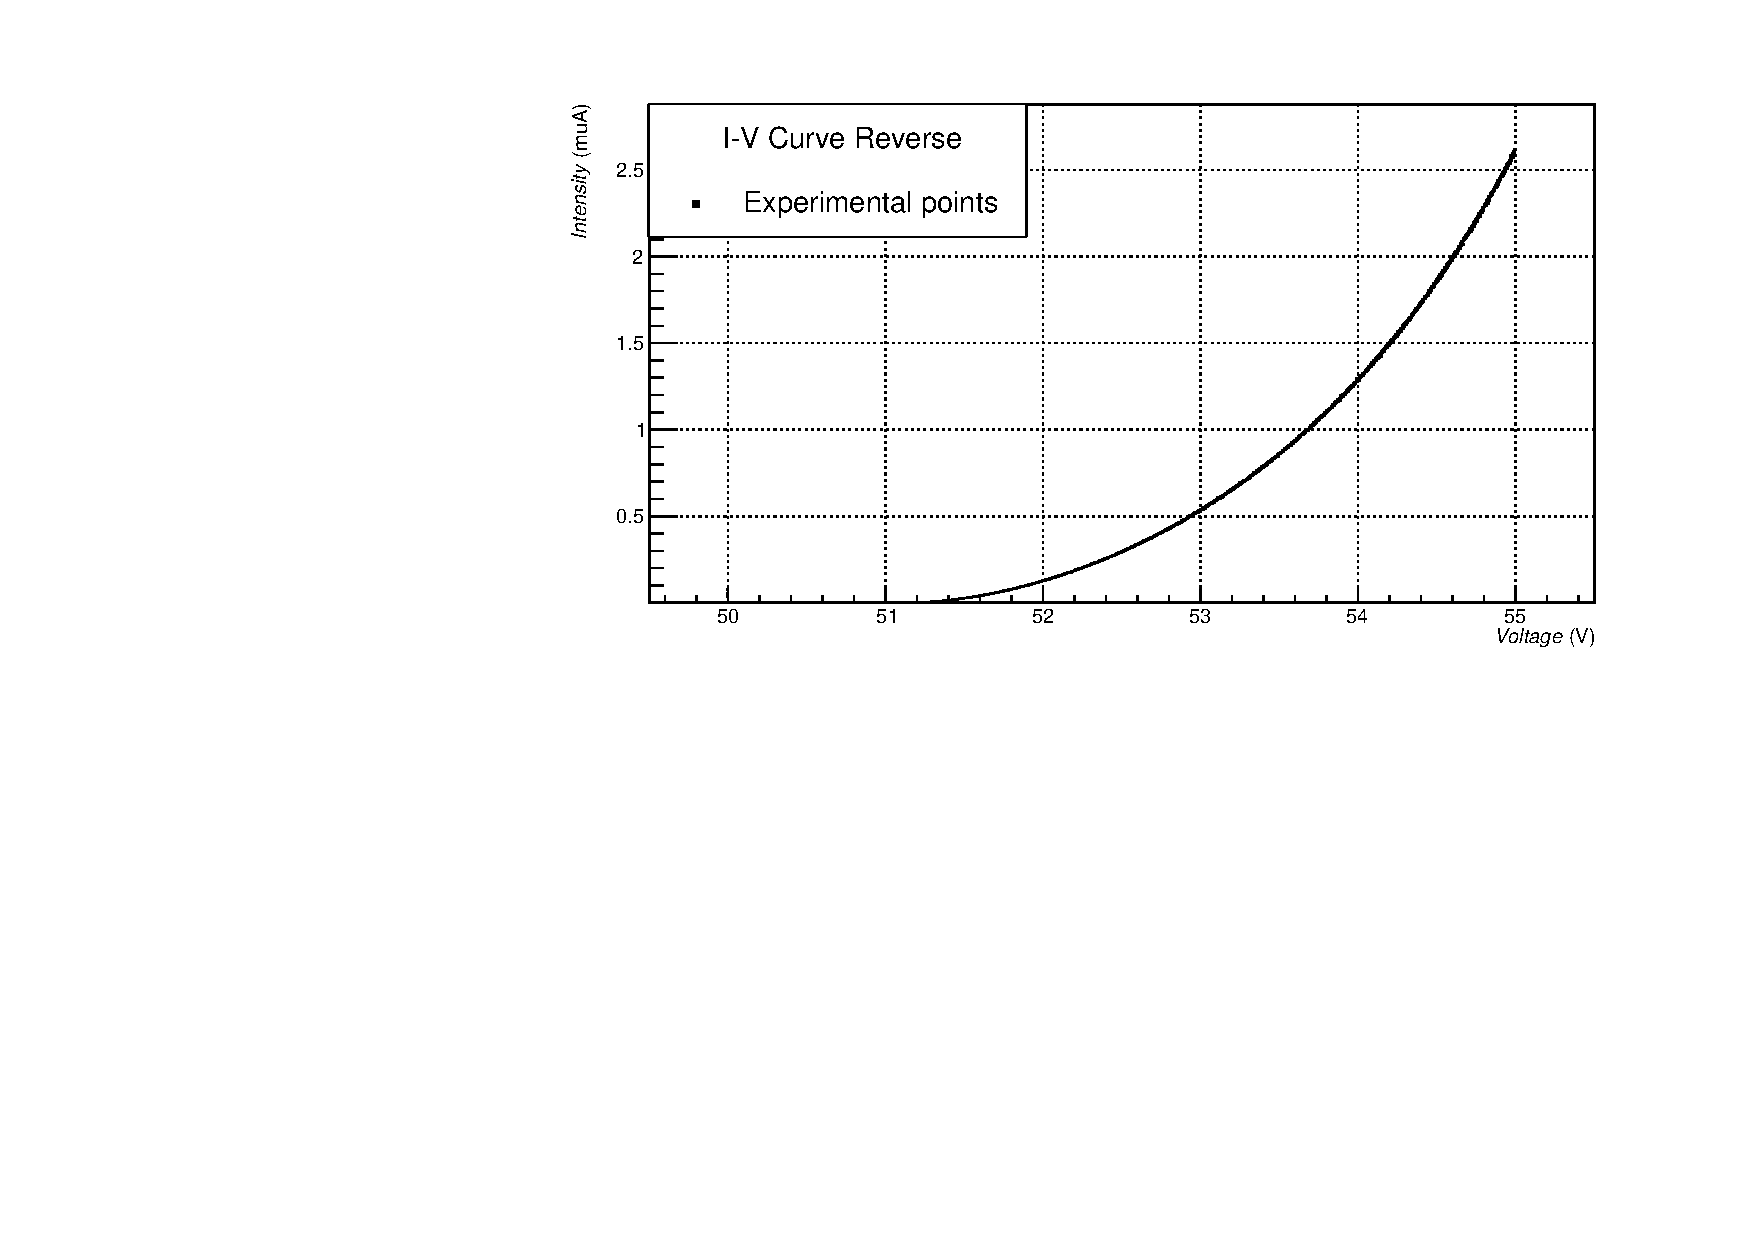
\includegraphics[width=\textwidth]{4ResearchAndDevelopments/42SiPM/IVCurveSiPMReverse.pdf}  
    \caption{\label{subfig:IVcurveReverse}}
    \end{subfigure}
 \caption{I-V curves measured for the S13360-1375 SiPM model from Hamamatsu a) Forward bias b) Reverse bias. The measurements were taken at $T=25\celsius$ and $H=45\%$.}
 \label{fig:IVcurveSiPM}
\end{figure}
As can be seen, when the SiPM is forward biased (Figure \ref{subfig:IVcurveForward}) there is no output current until a potential drop of $V_0= 0.5~\volt$ is reached. When the current starts to flow, the intensity is linear with the applied voltage. The equivalent resistance $R_{eq}$ was determined from, 
\begin{equation}
I=\frac{1}{R_{eq}}V;  \qquad \frac{1}{R_{eq}} = \sum_{i=1}^{N}\frac{1}{R_{q}}= \frac{N}{R_{q}}
\label{QuenchingResistance}
\end{equation}
and $R_{q}$ are the quenching resistance of a pixel. A value of $R_{q}= 360.56 \pm 0.07~\kilo\ohm$ was obtained from a linear fit to the data, which is in agreement with the typical values given by Hamamatsu. The breakdown voltage, $V_{BD}$, was obtained from the reverse bias voltage plot (Figure \ref{subfig:IVcurveReverse}). $V_{BD}$ is the point at which the SiPM begins to operate in avalanche mode for reverse bias. $V_{BD}$ is calculated from the maximum of the function 
\begin{equation}
f=\frac{1}{I}\frac{dI}{dV}
\label{BreakDownVoltageFunction}
\end{equation}
The value obtained $V_{BD}=51.02~\volt$ is in agreement with the value provided by Hamamatsu, given in Table \ref{tab:PropertiesOfSiPM1375}.

To measure the SiPM gain $G_{SiPM}$, the electronic board described in section \ref{sec:MonitorOverview} with an amplification factor of $F_{amp}=170$ was employed. An incoherent light source, LED435-03 \cite{LEDRLT}, described in section \ref{sec:CharacterizationScintillatingFibers}, was used to illuminate the SiPM with low enough flux intensities. The SiPM output signal shows various well-defined pulse heights, shown in Figure \ref{fig:OutputPulses_SPSspectrum}, corresponding to the number of pixels simultaneously fired. The single photon spectrum SPS is plotted in Figure \ref{fig:OutputPulses_SPSspectrum}. This spectrum was obtained by integrating and hitogramming the SiPM output pulses within a time window wide enough to contain the full charge of the pulse. The time window used in these measurements was $t_w= 500~\nano\second$. The light source provides a trigger signal for the measurement, represented in green line in Figure \ref{fig:OutputPulses_SPSspectrum}.
\begin{figure}[hbtp]
\centering
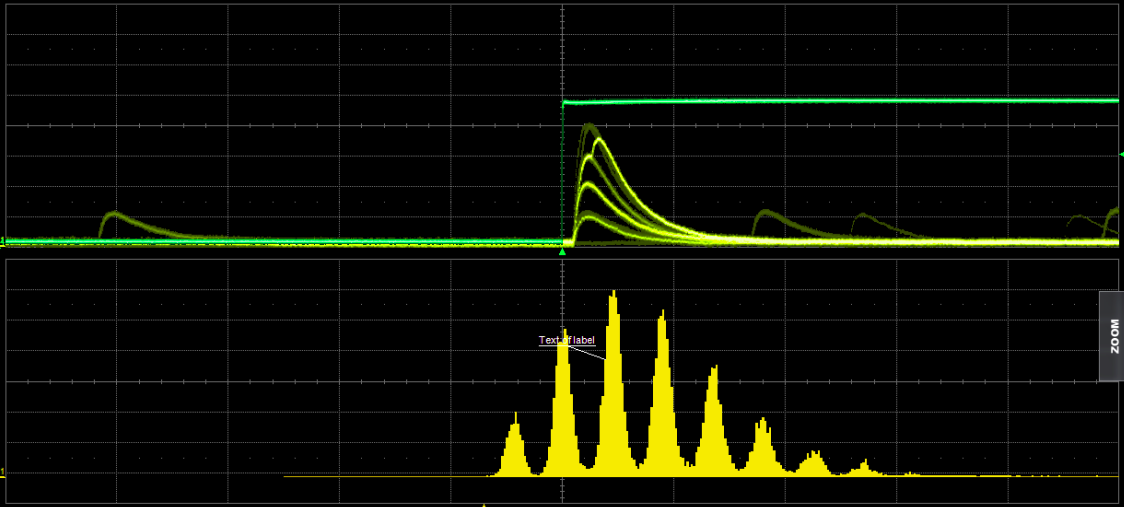
\includegraphics[scale=0.3]{4ResearchAndDevelopments/42SiPM/SiPMPulses_SPS_Spectrum.png}
\caption{Above) Trigger signal (green) and SiPM output pulses (yellow). Below) SPS spectrum obtained by integrating and histograming the SiPM output pulses. This measurement was done at $T=25\celsius$, $V_{bias}=53.98$ and $H=60\%$. \label{fig:OutputPulses_SPSspectrum}}
\end{figure}
The well-separated peaks in the SPS spectrum correspond to the charge produced by a different number of pixels fired. The first peak in the spectrum is the pedestal, which is the charge measured when no pixel is fired. This peak is caused by the electronic noise of the system. The second peak corresponds to one fired pixel and so on. The SiPM gain $G_{SiPM}$ can be obtained from the SPS spectrum from the equation,
\begin{equation}
G=\frac{\overline{\Delta Q}}{F_{amp} \times e}
\label{SiPMGain}
\end{equation}
where $e$ is the electron charge and $\overline{\Delta Q}$ is the average peak distance in the SPS spectrum, corresponding to the charge released by a fired pixel. 

To obtain the value of $\overline{\Delta Q}$, a macro was written in ROOT \cite{ROOTWebPage}. This macro extracts the bakcground (the pedestal substracted output signals when the SiPM is not illuminated), which is crucial in some cases like high temperatures or high bias voltages since background can hide peaks. After substracting the background, this macro find all peaks in the SPS spectrum and fits each one to a Gaussian funtion, as shown in Figure \ref{subfig:GaussianFitSiPMs}. The charge produced by multiple fired pixels is obtained from the centroid of the peaks. The charges fitted to the number of fired pixels is plotted in Figure \ref{subfig:LinearFitSiPMGain}.
\begin{figure}
\centering
    \begin{subfigure}[b]{0.9\textwidth}
    \centering
    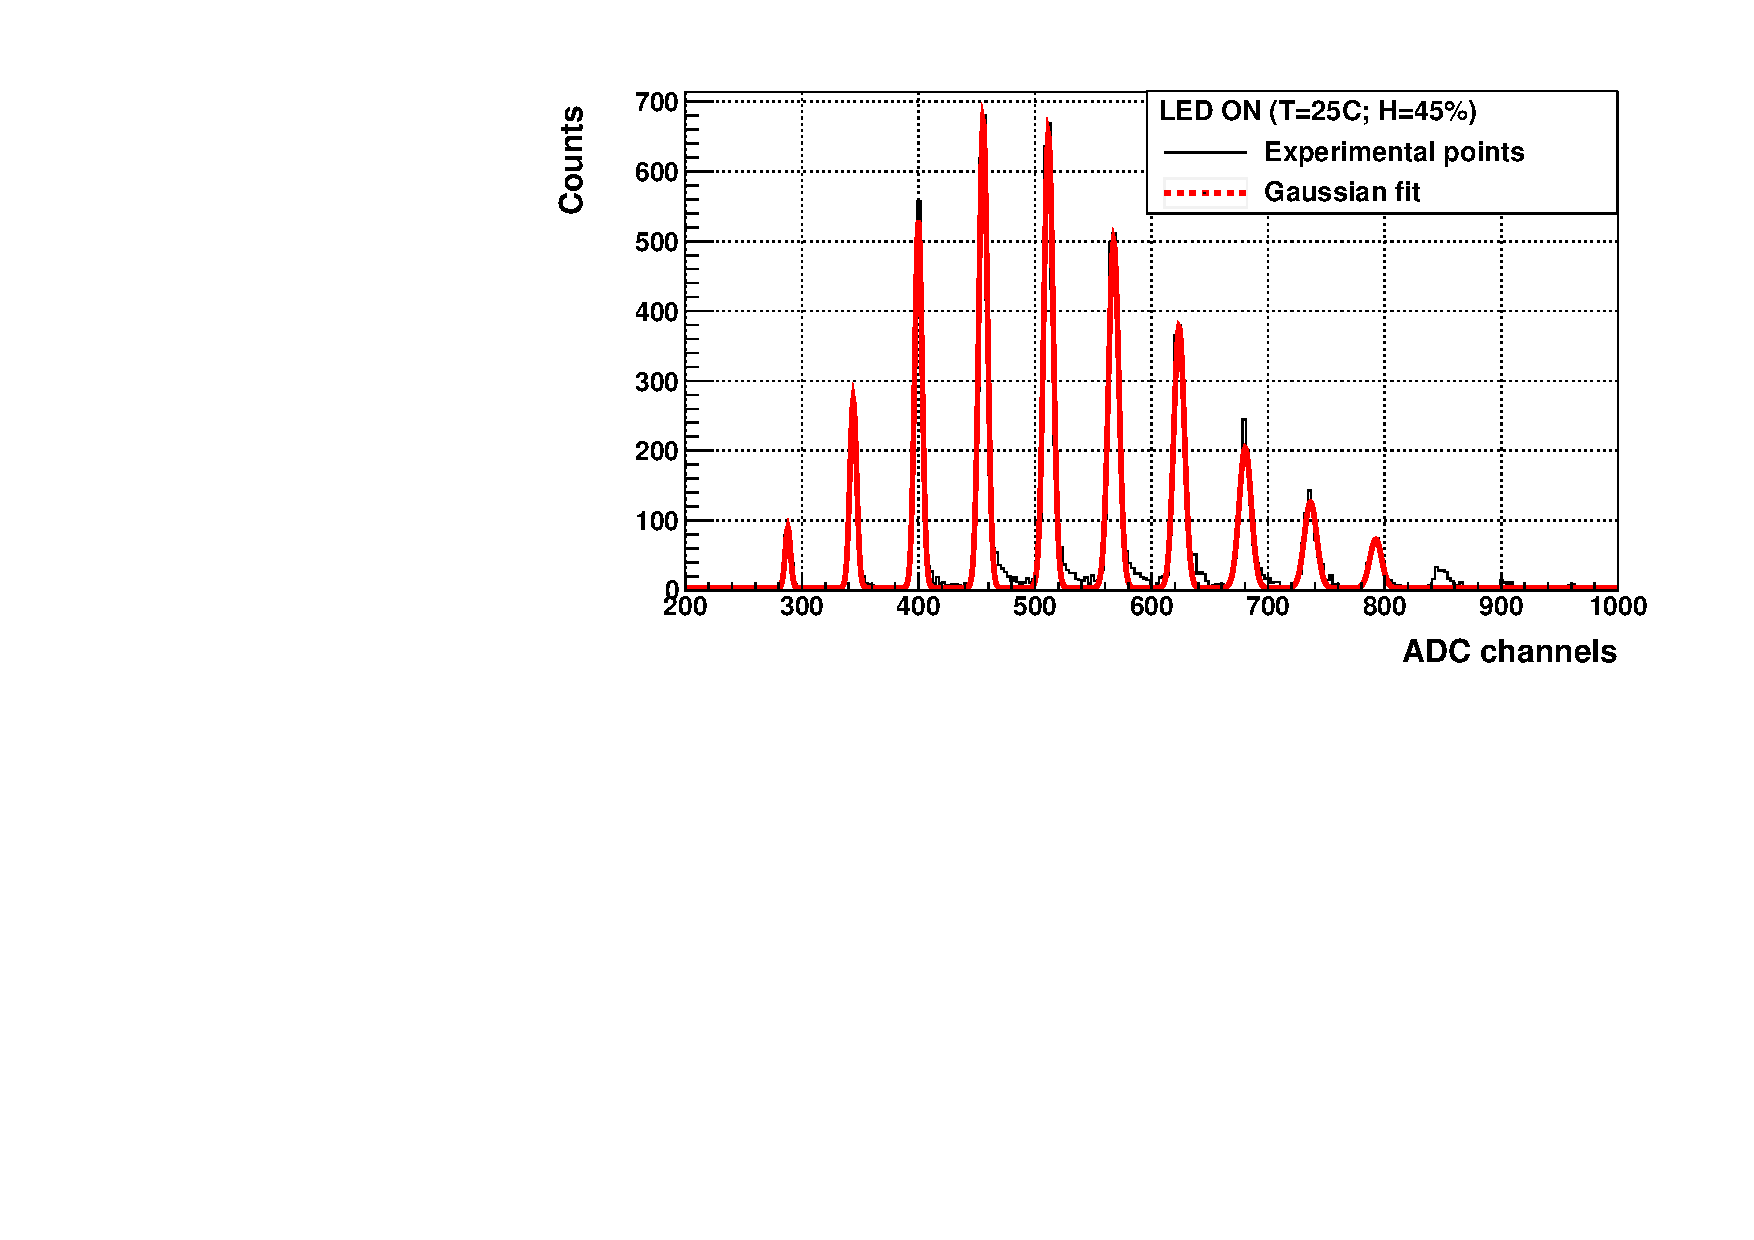
\includegraphics[width=\textwidth]{4ResearchAndDevelopments/42SiPM/GaussianFitSPSSpectrum.pdf}  
    \caption{\label{subfig:GaussianFitSiPMs}}
    \end{subfigure}
    \hfill
    \begin{subfigure}[b]{0.9\textwidth}
    \centering
    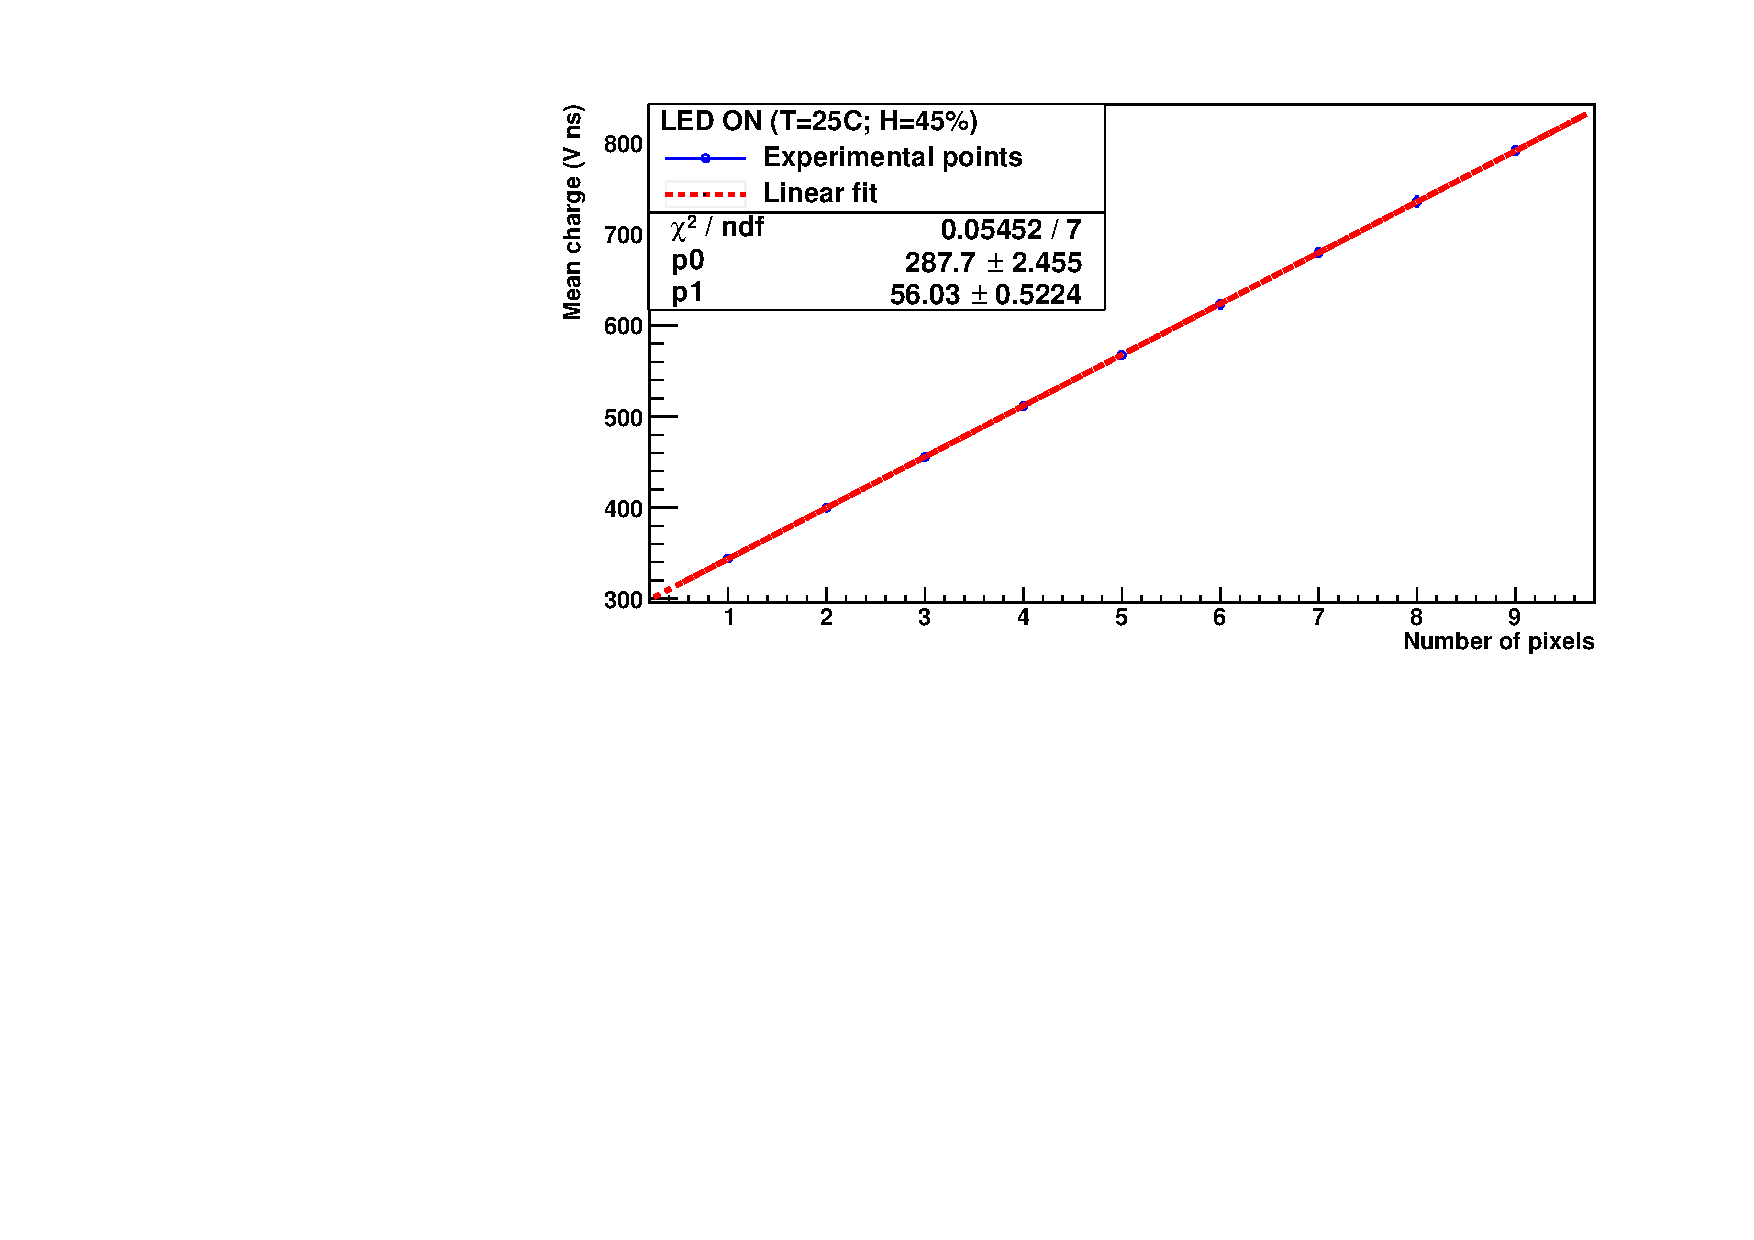
\includegraphics[width=\textwidth]{4ResearchAndDevelopments/42SiPM/LinearFit_Gain_NPixels.pdf}  
    \caption{\label{subfig:LinearFitSiPMGain}}
    \end{subfigure}
 \caption{a) Fit of the SPS spectrum to Gaussian functions. b) Charge as a function of the number of pixels fired. Error bars are within point size. Data taken at $T=25\celsius$, $V_{bias}=53.98~\volt$ and of $H=45\%$.}
 \label{fig:ROOTAnalysisSiPMGain}
\end{figure}
Up to 10 simultaneously fired pixels were obtained with a relative uncertainty of the charge measurement of less than $2\%$. The slope of the straight line in Figure \ref{subfig:LinearFitSiPMGain} corresponds to $\overline{\Delta Q}$.
For the case studied, which corresponds to a temperature of $25~\celsius$ and a bias voltage of $53.96~\volt$ (overvoltage around $3~\volt$), the value obtained for the SiPM gain is $G_{SiPM}=(4.11 \pm 0.04) \cdot{} 10^{6}$, very close to the data sheet value, given in Table \ref{tab:PropertiesOfSiPM1375}.

A method for SiPM gain stabilization against temperature was implemented. This is necessary for the TRITIUM project since the temperature in the final location of the tritium detector cannot be controlled with the sufficient accuracy to avoid significant variations of the SiPM gain. This method consists in compensating variations of the SiPM gain caused by temperature changes, by controlled modification of the bias voltage. For this task, the dependence of the SiPM gain with the temperature and bias voltage was measured. The SiPM gain was measured from $15\celsius$ to $41\celsius$ in steps of $2\celsius$, which is expected to be the temperature range in the final location. The bias voltage was $V_{bias} = V_{BD}+3$. The SiPM gain was measured at several overvoltages from $1~\volt$ to $5~\volt$ in steps of $0.2~\volt$. The temperature was $T=25\celsius$. Both measurements are shown in Figure \ref{fig:SiPMGainDependance}.\begin{figure}
\centering
    \begin{subfigure}[b]{0.9\textwidth}
    \centering
    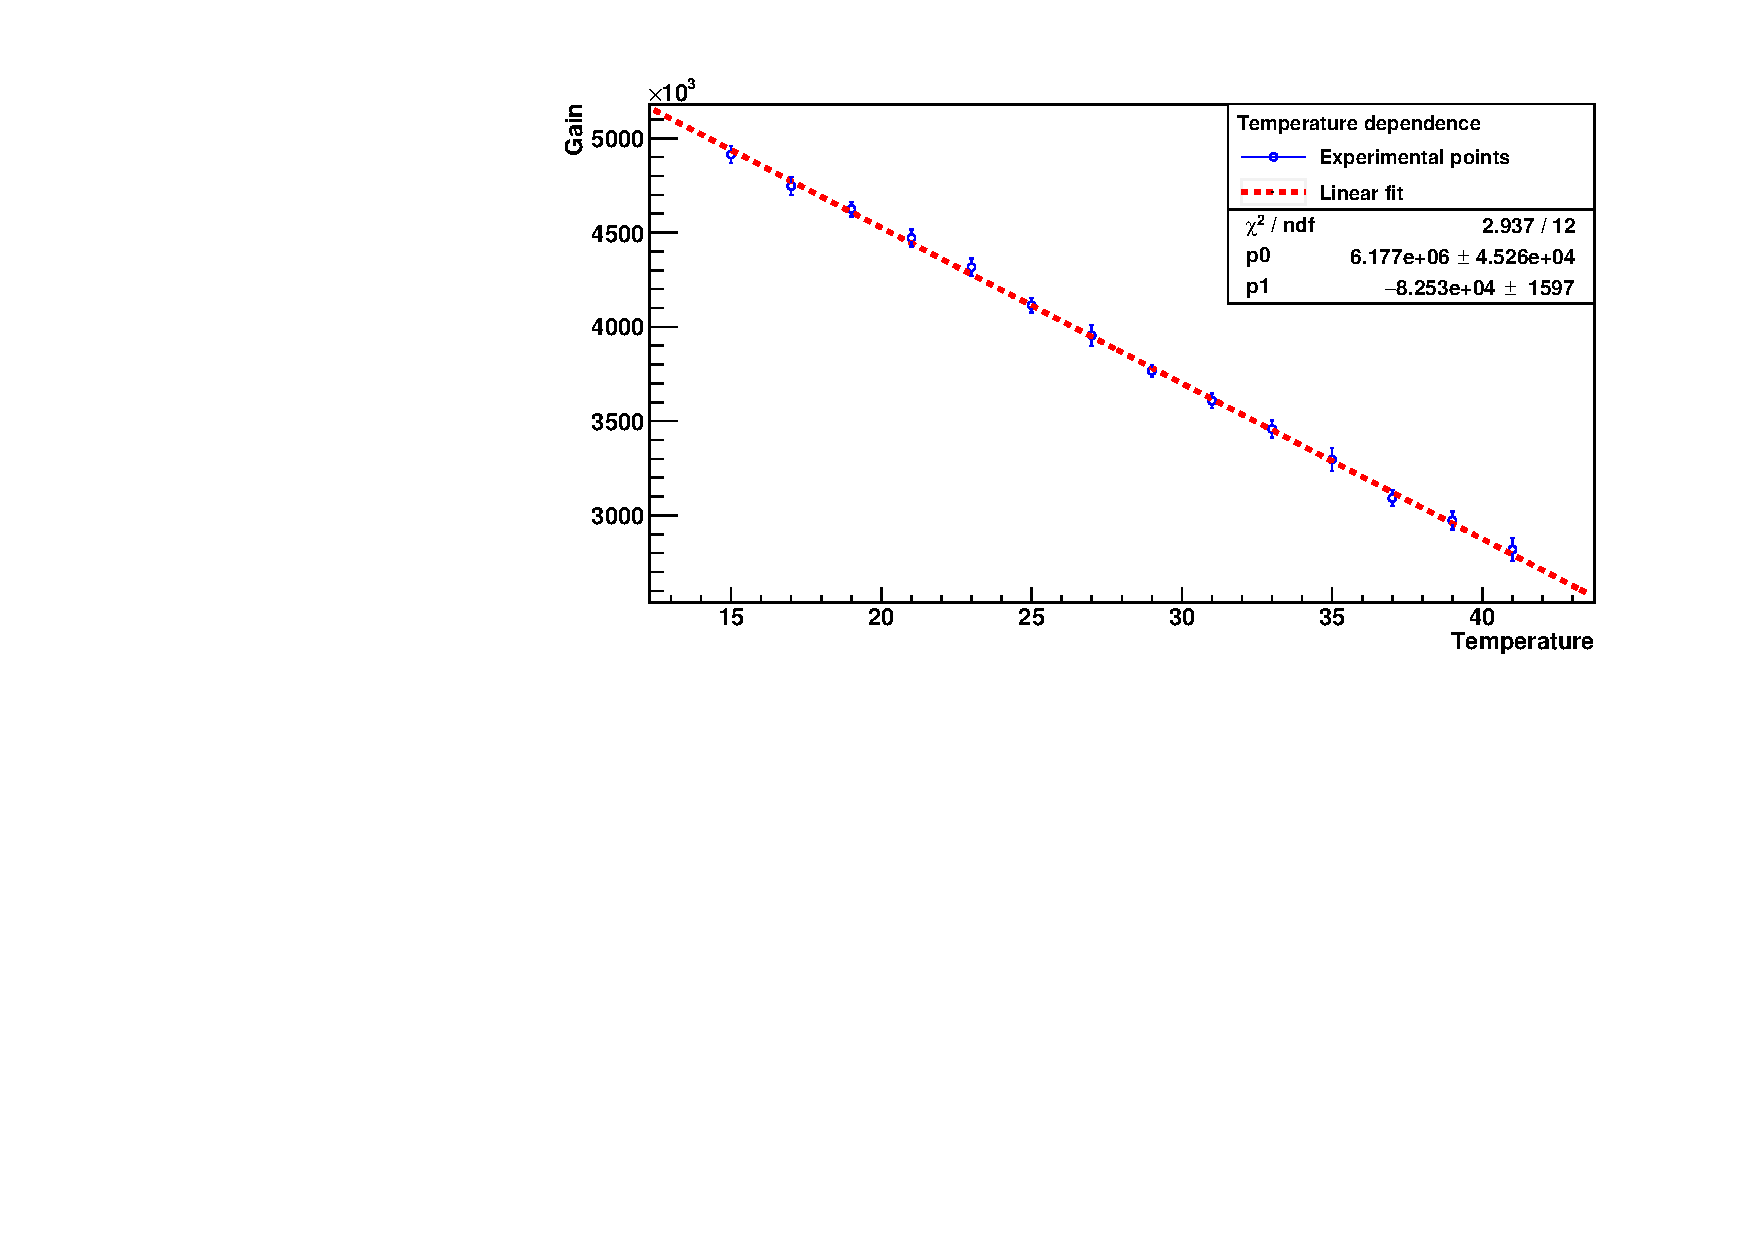
\includegraphics[width=\textwidth]{4ResearchAndDevelopments/42SiPM/SiPMGain_vs_Temperature.pdf}  
    \caption{\label{subfig:SiPMGainvsTemperature}}
    \end{subfigure}
    \hfill
    \begin{subfigure}[b]{0.9\textwidth}
    \centering
    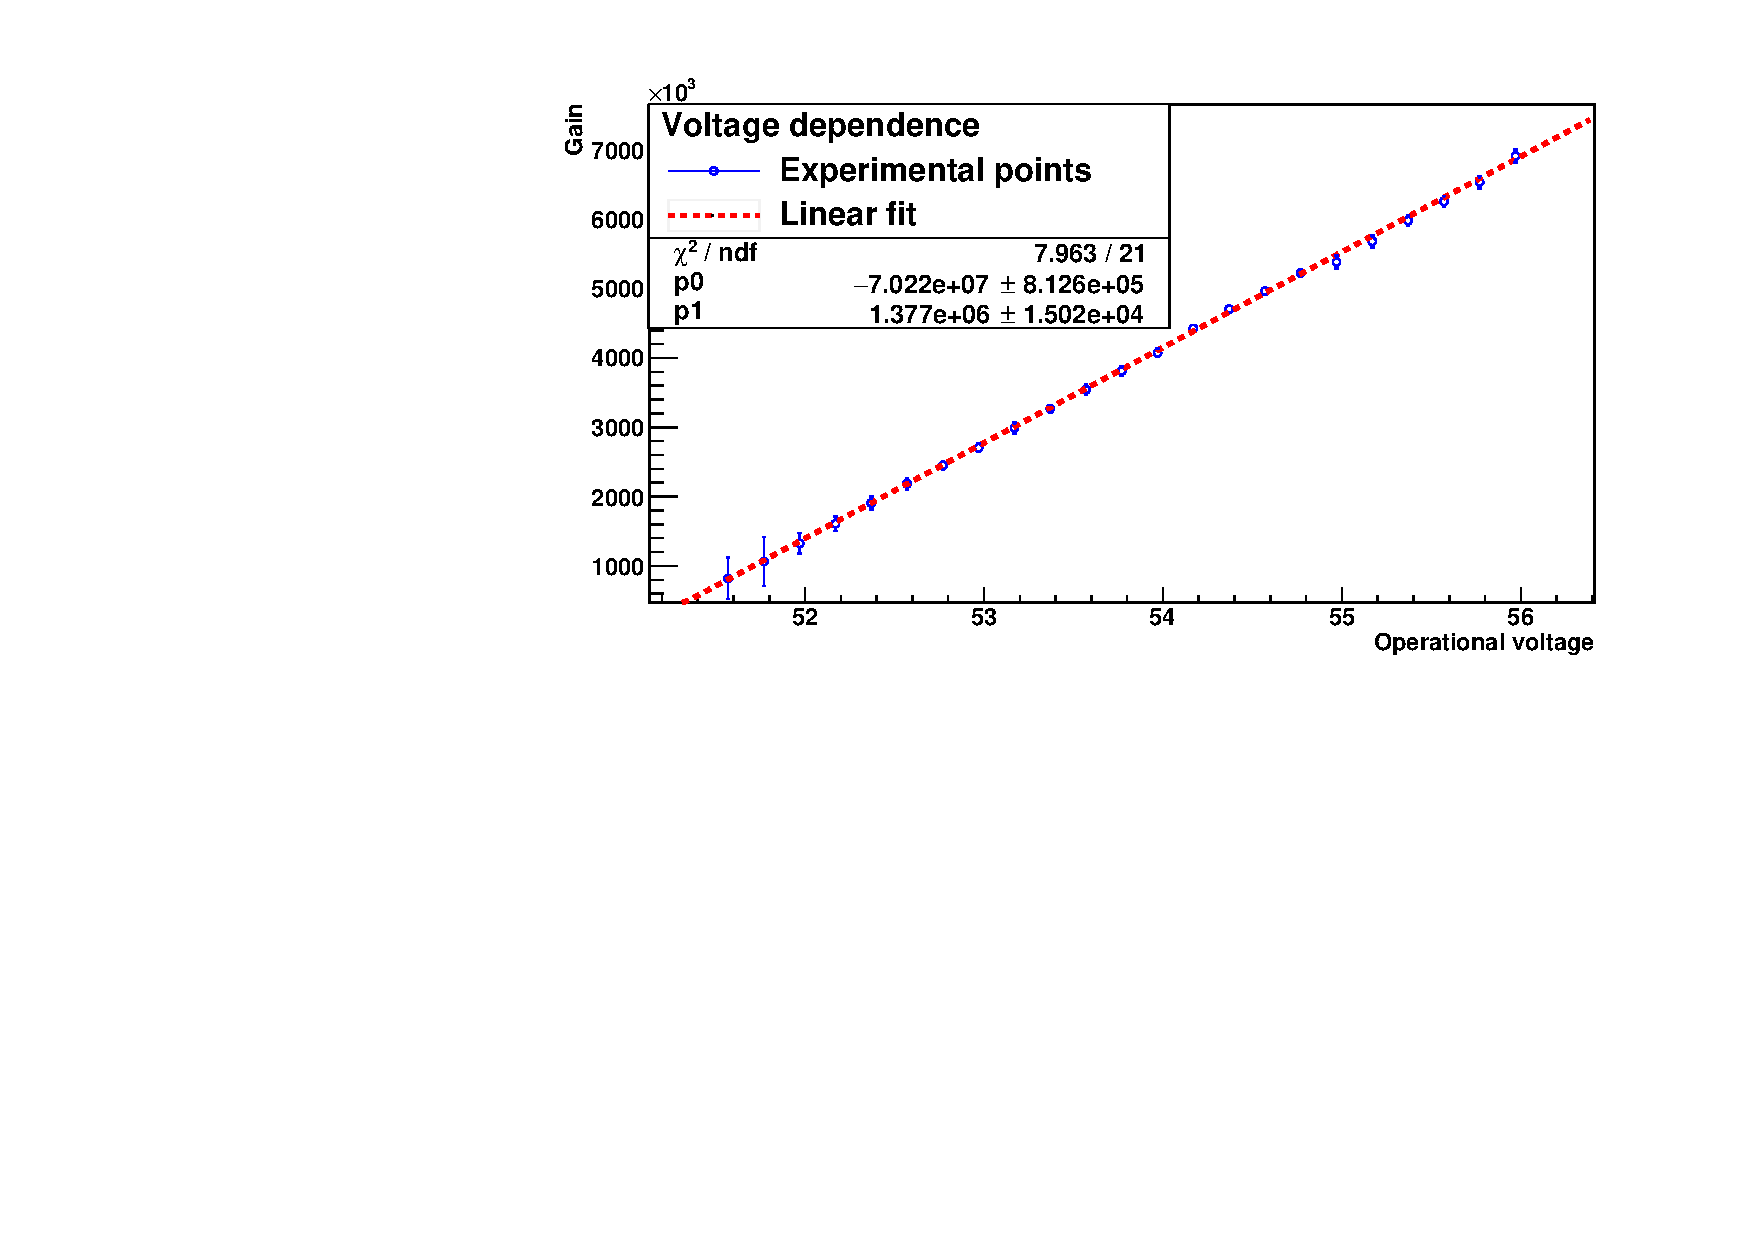
\includegraphics[width=\textwidth]{4ResearchAndDevelopments/42SiPM/SiPMGain_vs_Bias_Voltage.pdf}  
    \caption{\label{subfig:SiPMGainvsBiasVoltage}}
    \end{subfigure}
 \caption{SiPM gain versus a) Temperature. b) Bias voltage.}
 \label{fig:SiPMGainDependance}
\end{figure}
An excellent linear behaviour is obtained for both cases. From a linear fit, It is obtained,
\begin{equation*}
\begin{split}
G_{SiPM}=a \cdot{} T + b;& \qquad G_{SiPM}=c \cdot{} V_{bias} + d\\
a=\left( -82.5 \pm 1.6 \right) \cdot{} 10^{3};& \qquad c=\left( 137.7 \pm 1.5 \right) \cdot{} 10^{4}\\
b=\left( 618 \pm 5 \right) \cdot{} 10^{4};& \qquad d=\left( -762 \pm 8 \right) \cdot{} 10^{5} \\
\label{SiPMGainVSTempV}
\end{split}
\end{equation*} 
The breakdown voltage $V_{BD}$ and the terminal capacitance $C_t$ can be obtained from the linear fit of the SiPM gain versus the bias voltage $V_{bias}$,
\begin{equation}
G_{SiPM}=\frac{Q_{pixel}}{e} = C_d \frac{V_{bias}-V_{BD}}{e} = c \cdot{} V_{bias}+d
\label{SiPMGain_Capacitance}
\end{equation}
where $C_d$ is the pixel capacitance. From the linear fit of Figure \ref{subfig:SiPMGainvsBiasVoltage}, $V_{BD}=51 \pm 0.6~\volt$ and $C_d{}= 220.6 \pm 2.4~\text{f}\farad$ are obtained. The terminal capacitance of the SiPM is calculated as $C_{t}=N_{p} \cdot{} C_{d}=62.9 \pm 0.7~\pico\farad$. Both breakdown voltage and terminal capacitance, are in agreement with the values given in Table \ref{tab:PropertiesOfSiPM1375}. 

Finally, the bias voltage needed to compensate the variation of the SiPM gain due to temperature changes is obtained from the derivatives of the linear relations,
\begin{equation*}
\begin{split}
G_{SiPM}=a \cdot{} T + b  &\longrightarrow \partial G_{SiPM}= a \partial T\\
G_{SiPM}=c \cdot{} V_{bias} + d &\longrightarrow \partial G_{SiPM}= c \partial V_{bias}
\label{Gain_compensationVariations}
\end{split}
\end{equation*} 
The total variation of the SiPM gain produced by the variation of both $V_{bias}$ and $T$, must cancel,
\begin{equation*}
\begin{split}
d G_{SiPM, tot}= \frac{\partial G_{SiPM}}{\partial T} dT + \frac{\partial G_{SiPM}}{\partial V_{bias}} dV_{bias}& = a \cdot{} dT + c \cdot{} dV_{bias} = 0\\ 
dV_{bias}  = - \frac{a}{c}& dT = - e dT
\label{Gain_compensation0}
\end{split}
\end{equation*} 
where the parámeter $e= \frac{a}{c} 59.9 \pm 1.3~\milli\volt/\celsius $ agrees with the temperature coefficient provided in the data sheet, given in Table \ref{tab:PropertiesOfSiPM1375}. Converting the differentials in finite increments,
\begin{equation}
\begin{split}
\int_{V_i}^{V_f}\partial V_{bias}  = -e\int_{T_i}^{T_f}\partial T \longrightarrow \Delta V_{bias} = -e \Delta T
\label{Gain_compensationIntegring}
\end{split}
\end{equation} 
gives the variation of the voltage $\Delta V_{bias}$ that keeps constant the SiPM gain for a variation in temperature, $\Delta T$. To know the bias voltage $V_{bias}$ to be applied as a function of the temperature $T$ a reference value is needed. The reference considered is $V_{ref}= V_{BD}+3~\volt = 53.98~\volt$ and $T_i=T_{ref}=24\celsius$, at which the measured gain is $4.2 \cdot{} 10^{6}$. Thus, we get:
\begin{equation*}
\begin{split}
(V_{bias}-V_{ref} )= e \left( T -T_{ref} \right) 
\label{Gain_compensationEquation}
\end{split}
\end{equation*}
\begin{equation}
V_{bias}(\volt)= 59.93 \cdot{} 10^{-3} \cdot{} T(\celsius) + 52.54
\label{Gain_compensationReference}
\end{equation}  
To test the bias voltage compensation, the temperature was varied from $21\celsius$ to $29\celsius$ and the bias voltage was modified according to the equation \ref{Gain_compensationReference}. The value of the SiPM gain obtained as a function of the temperature is shown in Figure \ref{fig:SiPMGainStabilization}.

\begin{figure}[hbtp]
\centering
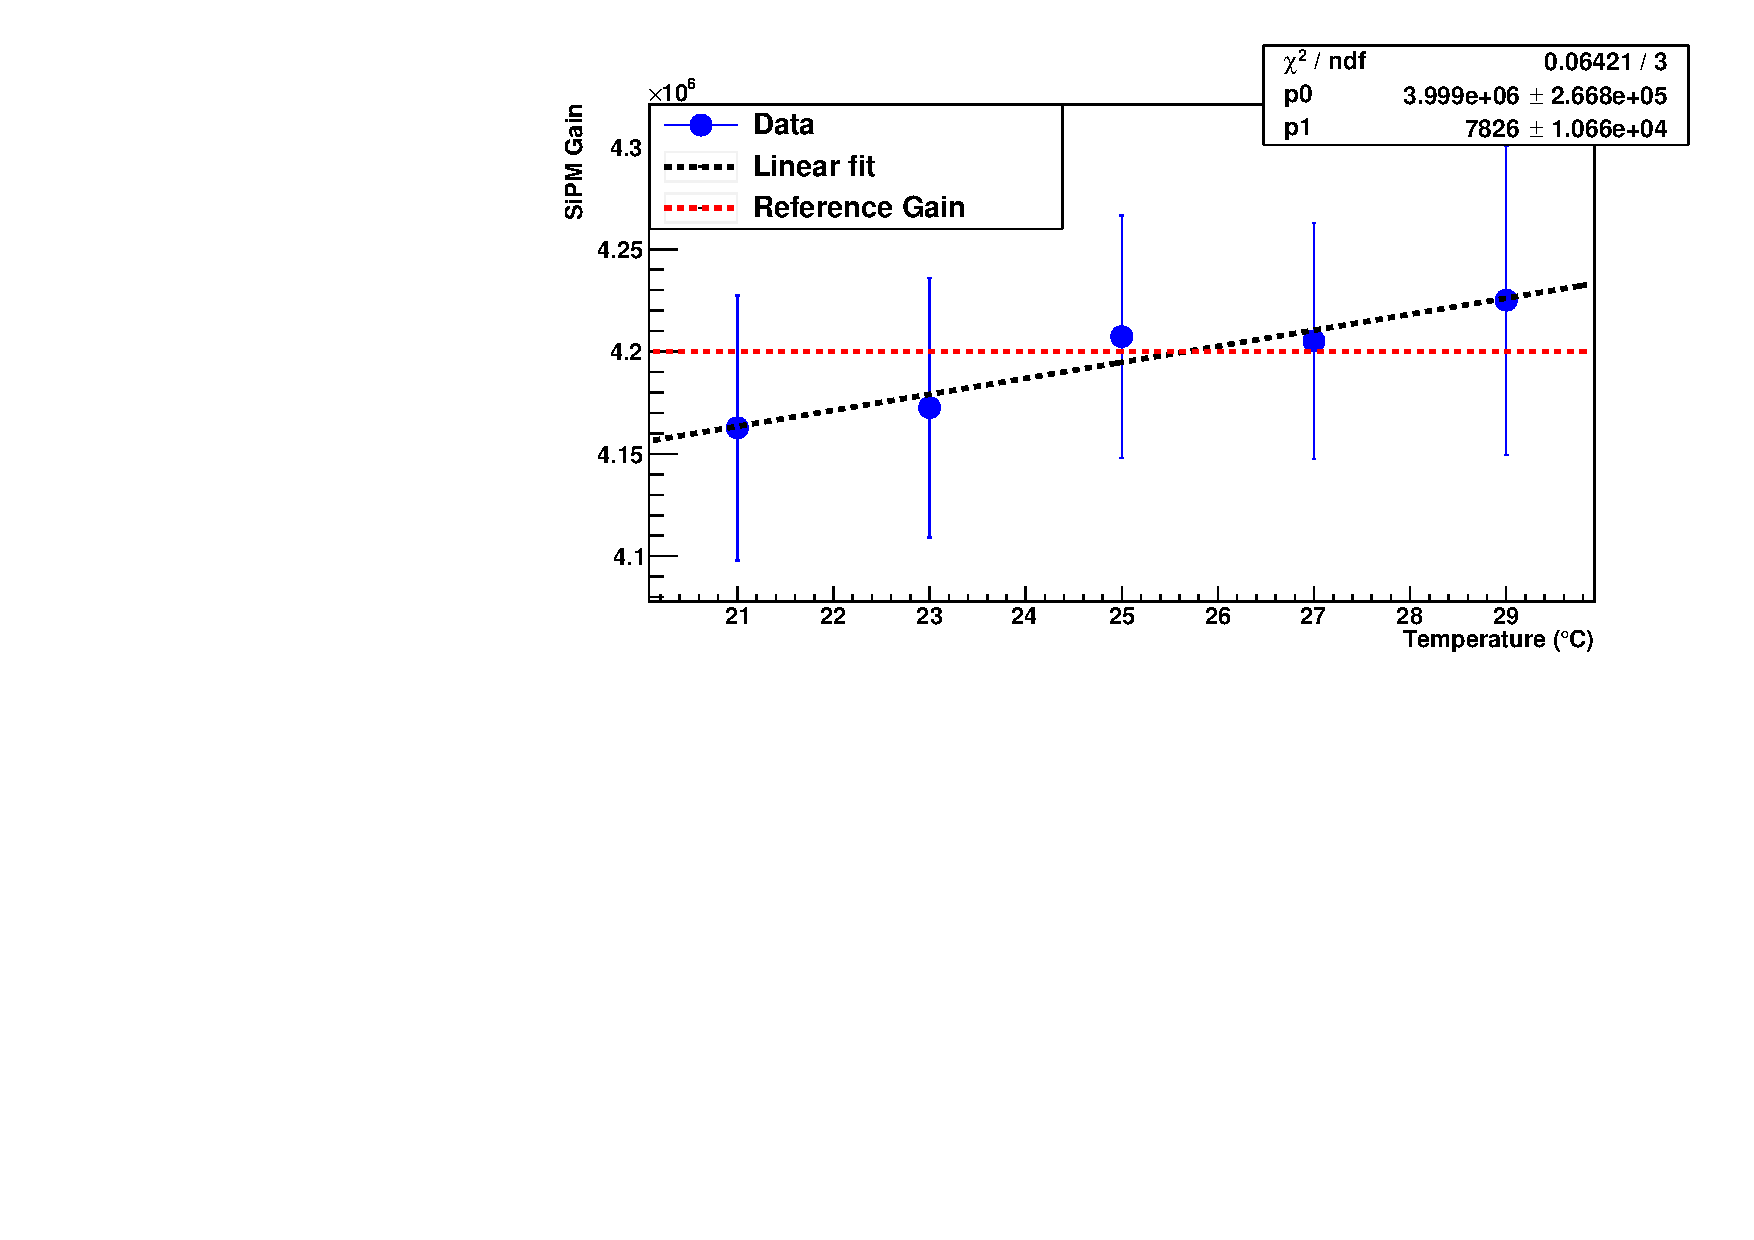
\includegraphics[scale=0.75]{4ResearchAndDevelopments/42SiPM/SiPMGain_Stabilization_linear_fit.pdf}
\caption{SiPM gain as a function of the temperature after implementation of the gain stabilization method. \label{fig:SiPMGainStabilization}}
\end{figure}
The red dotted line indicates the reference SiPM gain. As it can be seen, the gain variation with temperature is reduced to $0.25\%\celsius^{-1}$ with is negligible. Furthermore, all measured points are in agreement with the initially value measured for the SiPM gain. Therefore, this method stabilizes the gain of the SiPM against temperature variations.